\documentclass[a4paper,3p,sort&compress]{elsarticle}

\usepackage[draft]{hyperref}
\usepackage{url}
\usepackage{booktabs}
\usepackage{graphicx}
\usepackage{xspace} 
\usepackage{booktabs}
\usepackage{makecell}
\usepackage{lineno}
\usepackage{natbib}
\usepackage{amsmath}
\DeclareRobustCommand{\citeext}[1]{\citeauthor{#1}~\cite{#1}}

\usepackage[nomargin,inline,draft]{fixme}
\fxsetup{theme=color,mode=multiuser}
\FXRegisterAuthor{j}{jla}{\color{purple}JLA}
\FXRegisterAuthor{s}{spv}{\color{teal}SPV}

\journal{-}

%% `Elsevier LaTeX' style
\bibliographystyle{plain}
%%%%%%%%%%%%%%%%%%%%%%%

\begin{document}
\linenumbers

% Macro para escribir NO$_2$
\newcommand{\no}{NO\textsubscript{2}\xspace}

\begin{frontmatter}

  \title{Pollution Forecast: Introducing a novel visualization technique for time series uncertainty visualization}


  \author{Sebasti\'an P\'erez Vasseur}
  \author{Jos\'e L. Aznarte}
  \address{Artificial Intelligence Department\\Universidad Nacional de
    Educaci\'on a Distancia --- UNED\\c/ Juan del Rosal, 16, Madrid, Spain}
  \ead{jlaznarte@dia.uned.es}
  

\begin{abstract}
  
\end{abstract}

\begin{keyword}
probabilistic forecasting \sep visualization \sep dotplot
\end{keyword}

\end{frontmatter}

%\linenumbers

\section{Introduction}
\label{sec:intro}

Uncertainty is an inherent part of data analysis and decision making and its correct estimation 
is necessary to estimate risks and possible outcomes. For example, Rouston et al. showed that 
in the case of weather forecasts, analysts could improve their rewards and reduce their exposure 
to risk thanks to the presented uncertainty. In this paper, we define uncertainty as the probability 
distribution of a numeric value.

However, uncertainty visualization and understanding has faced many challenges. 

As Padilla et al. points out, this could be due not only by the abstract nature of probability 
but also to poor communication techniques. Weiskopf et al. reaches a similar conclusion and states 
that uncertainty communication should be linked to the way it is communicated.

For instance, one of the most typical approaches, Visual Boundaries such as isocontours and error 
bars display value areas within a certain  confidence interval. The problem with this approach is 
that individuals may exclude as possible values outside the confidence interval, which are still 
plausible, only less probable. 

Also, Bella et al showed that leading researchers had trouble reading error bars and they confused 
standard errors and confidence intervals. 

However, Joslyn and LeClerc showed that individuals could also be inclined to take uncertain 
information as deterministic, for example by considering the confidence interval for wether temperature 
forecast as high and low temperature.

As noted by Josly et al., this has lead to a new surge of research in visualization techniques: Van 
der Bles et al. point that there is more than error bars to show uncertainty. 

One possible solution to this problem is the use of HOPs (hypothetical outcome plot). HOPs display 
random draws from a distribution and animate the draws over time. However, this technique can not be 
applied to static visualizations. 

An alternative approach, Visual Semiotics uses visual encoding such as fuzziness or color to represent 
the probability of a certain value. An example of this would be the use of gradients to represent the 
full probabiliity distribution. Neverthless, this type of encoding makes it difficult to read specific 
values. Finally, Frequency Framing uses natural frequencies to display probabilities. As noted by Gerd 
Gigerenzer, individuals prefer frequencies or ratio, like 1/10, when understanding probability. This has 
lead to the development of the quantile dot plot. The quantile dot plot, created by Kay et al. represents 
the probability distribution with dots: each dot represents 5\% probability and are sampled proportional 
to the quantiles of the distribution. Quantiles dot plot have proved to lead to better distribution 
understanding and probability estimates reading.

An important field on uncertainty is the uncertainty in time series: For instance, time series forecasting 
produces a time series with uncertainty that is used by analyst to take decisions.

Communication of uncertainty in time series involves showing the evolution of uncertainty in time: this 
is specially challenging as a visualization must display several distributions in a constrained space.  
As pointed out by Leffrang et al., not much research has been applied to the field of uncertainty visualization 
in the field of time series. However, we can see already solutions for this problem as confidence interval charts,
 time box plots or gradient charts. Nonetheless, those solutions have not been properly compared in terms of 
 probability reading and estimation. Also, we have not seen yet a solution involving frequency framing.

Therefore, this paper presents the results of a comparison in terms of probability reading between 4 different 
uncertainty visualization techniques confidence interval, time series box plot, visual semiotics and a 
novel technique using frequency framing. We will use air quality probabilistic forecasting as the ground 
for the comparisons.

\section{Time Series probabilistic charts} 
\label{sec:time_series}

The confidence interval chart shows in a line the evolution of the mean of the distribution
 over time alongside 2 lines: the evolution of the 5\% and 95\% percentile of the distribution. 
 User estimates the probabilities with the distance of the points to those lines.

The box plot chart shows different percentile with “boxes”. For each point in time, a white 
line shows the location of mean, then a rectangle (or box) lower and upper part will be located 
at the 25\% and 75\% percentile respectively, a narrower box upper and lower part will show 
the 5\% and 95\% percentile and finally a line’s edge will show the 1\% and 99\% percentile. 
This visual boundary representation shows more percentile than the confidence interval and 
is recommended when the distribution is not symmetrical and to show the edges of the distribution.

The gradient chart shows the evolution of the mean in a line and then displays areas whose 
color changes as we get further from the mean. We end up having an area with a gradient 
delimited by 2 lines: the 1\% and 99\% percentile. This representation allows to have the
 full range of percentiles represented.

Finally, the time series dot plot is a novel technique based on frequency framing. First, 
it shows the evolution of the mean of the distribution in a line. And then, for each time 
step, a circle for each decile is drawn: this way, we can estimate the percentage 
probability of being in an interval as 10 times the number of circles in that interval. 
This technique has 
specifically been designed for readability and although it displays less information than 
the gradient chart for instance, is much more readable.

This chart would draw a dot for each of the deciles of the target variable. This simplifies the 
readability of the chart as users just need to count the number of dots to estimate approximately 
the natural frequencies.

Figure \ref{figure:charts} shows a summary of those probabilistic time series charts.

\begin{figure}
  \centering
  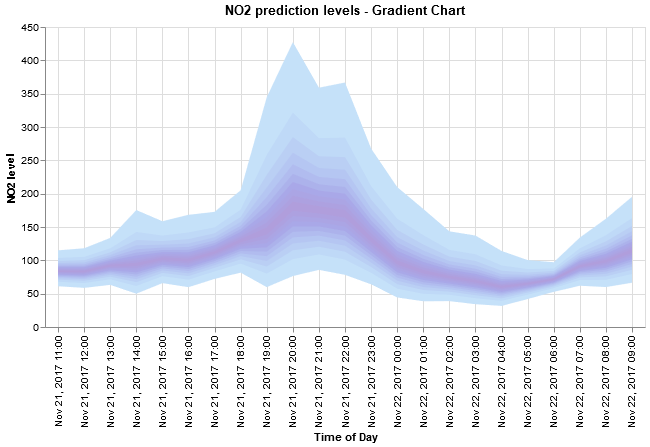
\includegraphics[width=0.4\textwidth]{gradient} 
  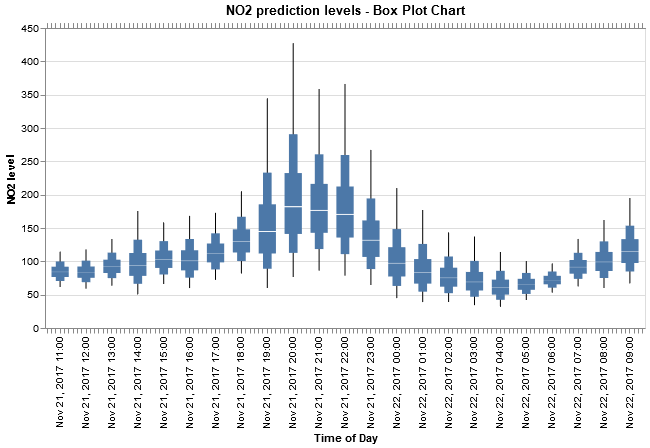
\includegraphics[width=0.4\textwidth]{boxplot}
  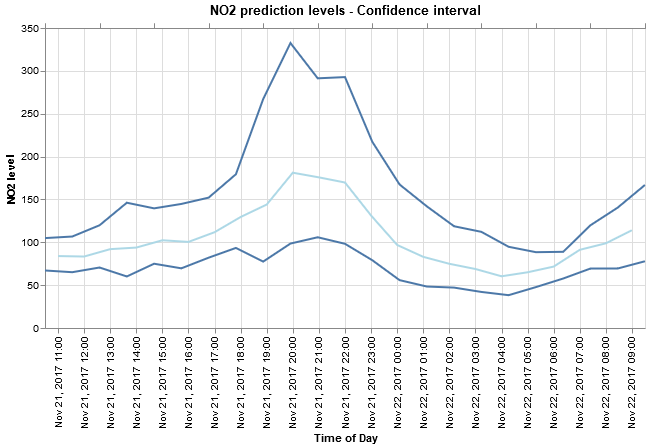
\includegraphics[width=0.4\textwidth]{ci} 
  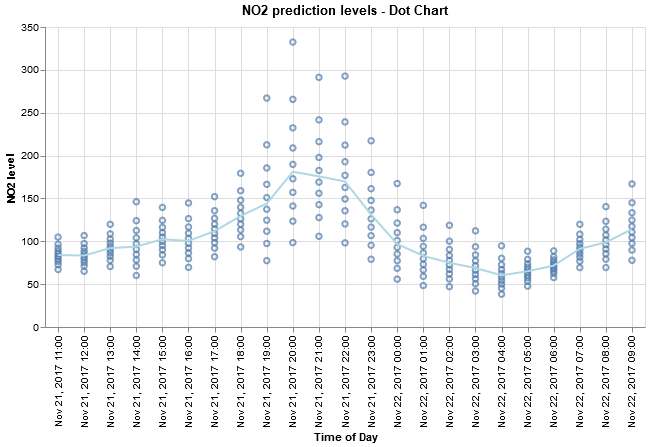
\includegraphics[width=0.4\textwidth]{dot}
  \caption{\label{figure:charts} Probabilistic Time Series Chart. 
  Top Left: Gradient Chart. Top Right: Box Plot. 
  Bottom Left: Confidence Interval. Bottom Right: Dot Chart.  }
\end{figure}

\section{Experimental Design}
\label{sec:exp_design}

We would like to compare the readability of the four main types of probabilistic time series charts displayed in figure 
\ref{figure:charts}. We will evaluate how well the charts can help answering a probability question regarding the NO levels.

For this, we will request the participation of users through the Amazon Mechanical Turk website. Those users will perform a small task
in exchange for a small fee (few dollars): the assigned task is a test where we measure how well can the participants read the charts.
As suggested by Brenner et al., we will be selecting Masters Level Participants. We will be testing 20 users per type of chart 
and as each is answering 5 questions, we will have 100 answers per type of chart.

For each type of chart, we designed a test with a presentation part where we explain how the charts can be read and a questions part
with 5 probability questions. As an example, we show in figure \ref{figure:explanation} the presentation part of the time series 
dot chart. The questions
require reading the chart to estimate the probability of the NO levels inside a certain range. We will then measure for each question
the error in the estimation and the time it took to answer. Inspired by the work of Brenner et al., we are also asking at the end of 
the survey how difficult was reading the chart and how confident are they with their answers. 

\begin{figure}
  \centering
  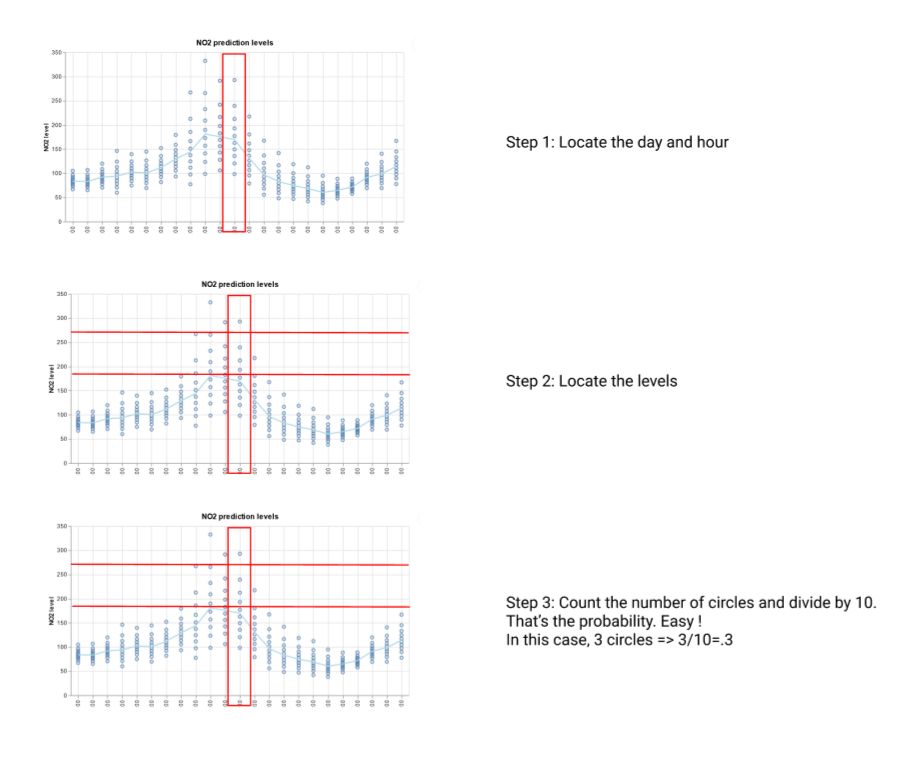
\includegraphics[width=0.8\textwidth]{dot_explanation}
  \caption{\label{figure:explanation} Image explaining how the chart is read.  }
\end{figure}  

\section{Results}
\label{sec:results}

Figure \ref{figure:errors} shows the histogram of the absolute value of the probability errors in percentage. 
Although the majority 
of users report errors on the 0-20\% section, the dot chart almost has no errors outside of this band. 
Also, we did not see an improvement in 
the error rate as users were answering questions, therefore we combined all errors together.

\begin{figure}
  \centering
  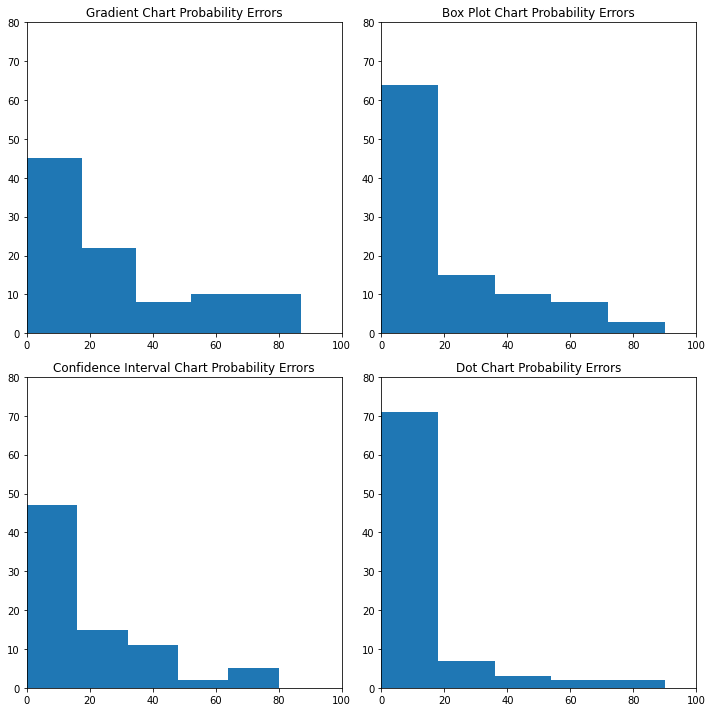
\includegraphics[width=0.6\textwidth]{probability_errors}
  \caption{\label{figure:errors}Distribution of absolute error for all questions per type of chart.}
\end{figure}

However, users seem to reflect their learning in the time it takes to read 
and answer the question. we see in figure \ref{figure:duration} that for every chart, the time it takes 
to read and answer the question decreases for every question answered. We also did not see 
noticeable difference between the type of charts. However, the difficulty of reading the chart might impact 
this number for a higher number of questions.

\begin{figure}
  \centering
   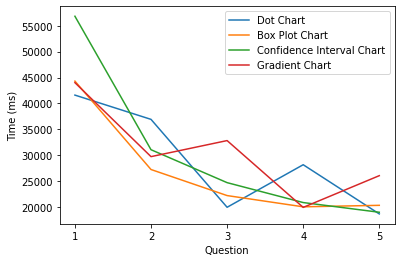
\includegraphics[width=0.6\textwidth]{duration_evo}
  \caption{\label{figure:duration} Median Time it took to answer each question for each of the types of chart.}
\end{figure}  

Confidence and load also prove the superior performance of the time series dot chart. 
Figure \ref{figure:confi_load} shows how the dot chart reports higher levels of confidence and 
lower levels of load of difficulty.

\begin{figure}
  \centering
   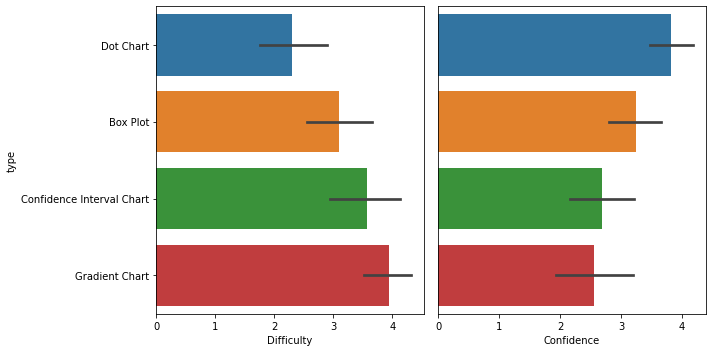
\includegraphics[width=0.5\textwidth]{confi_load}
  \caption{\label{figure:confi_load} Difficulty (left) and Confidence (right) in reading and answering the questions for each chart}
\end{figure}

We also see a lack of statistical knowledge from standard users as some users were reporting 
probabilities above 1, showing they do not understand the basic theory of statistics. 
We reported 9 users from 80 whose answers could not be used as their answers could not be 
applicable (probability higher than 1 or text).

\section{Conclusions}
\label{sec:concl}

We have compared 4 probabilistic time 
series charts when answering a quantitative probability question: 
gradient time series chart, box plot time series chart, confidence interval 
time series chart and time series dot chart.
We have applied them to the field of \no pollution levels probabilistic 
time series as an application example and to build the user tests.
We enrolled a panel of volunteers and asked them to read the charts 
and determine the probability of \no to be in a certain interval at a certain 
hour.
All users learned to use the charts and after 5 questions all charts 
need almost the same amount 
of time to be read.
However, the results show that users have the highest accuracy when using 
the time series dot chart. Also this chart represents the easiest method 
to get the answer while also providing the highest confidence in the answer.


\section{References}
\label{sec:ref}


\bibliography{refs}

\end{document} 

